\documentclass[10pt, a4paper]{article}
% \usepackage[english]{babel}
\usepackage[brazilian]{babel}
\usepackage[utf8]{inputenc}
% \usepackage[T1]{fontenc}
\usepackage{lipsum}

% code
\usepackage{pythonhighlight}
\renewcommand{\lstlistingname}{Anexo} % Listing->Code
\usepackage{adjustbox}

% For subfigure use
\usepackage[font=small,labelfont=bf]{caption}
\usepackage{subcaption}

% Set page size and margins
% Replace `letterpaper' with`a4paper' for UK/EU standard size
\usepackage[a4paper,top=2cm,bottom=2cm,left=2cm,right=2cm,marginparwidth=2cm]{geometry}

% tabelas
\usepackage{array}
\usepackage{tabularx}
\usepackage{booktabs}

\usepackage{float}

% Useful packages
\usepackage{amsmath}
\usepackage{enumerate}

\usepackage{graphicx}
\usepackage[colorlinks=true, allcolors=blue]{hyperref}
\usepackage{cleveref}
%\usepackage[notransparent]{svg}
\newcommand{\crefrangeconjunction}{--}


\begin{document}

\def\TITLE{Lista 02}
\def\DISCIPLINE{MEC 2403 - Otimização e Algoritmos para Engenharia Mecânica}
\def\PROFESSOR{Ivan Menezes}
\def\AUTHOR{Pedro Henrique Cardoso Paulo}
\def\CONTACT{pedrorjpaulo.phcp@gmail.com}
\def\DATE{abril de 2023}

\title{\textbf{\TITLE} \\ \DISCIPLINE}
\author{\AUTHOR}
\date{\DATE}

\begin{titlepage}
      \begin{center}
          \vspace*{1cm}

          \Huge
          \textbf{\TITLE}

          \vspace{0.5cm}
          \LARGE
          \DISCIPLINE

          \vspace{1.5cm}

          \textbf{\AUTHOR \\ {\tt \CONTACT}}

          \vfill
          Professor: \PROFESSOR

          \vspace{0.8cm}

          
\includegraphics[width=0.2\textwidth]{../general/puc.jpg}

          \Large
          Departamento de Engenharia Mecânica\\
          PUC-RJ Pontifícia Universidade Católica do Rio de Janeiro\\
          \DATE

      \end{center}
  \end{titlepage}

\maketitle

\section{Introdução}

\subsection{Objetivos}

Esse é o entregável da \TITLE \ da disciplina \DISCIPLINE. Esse trabalho tem como objetivos:

\begin{enumerate}
  \item Implementar os principais métodos para cálculo de ponto de mínimo em funções de uma variável
  \item Aplicar esses métodos em funções 2D ao longo de uma dada direção
  \item Exercitar a linguagem de programação e as ferramentas de visualização gráfica
\end{enumerate}

\subsection{Links úteis}\label{links}

Nesta seção são listados alguns links e referências úteis para se entender o trabalho desempenhado.

\begin{enumerate}
  \item \href{https://web.tecgraf.puc-rio.br/~ivan/MEC2403/ProgMatematica_VazPereiraMenezes-Ago2012.pdf}{Apostila de programação matemática da disciplina}
  \item \href{https://github.com/prj-phcp/MEC2403_Activities}{GitHub usado para essa disciplina}
  \item \href{https://github.com/prj-phcp/MEC2403_Activities/blob/master/Lista2/Lista2.ipynb}{Notebook com o código para as figuras desse relatório}
  \item \href{https://github.com/prj-phcp/MEC2403_Activities/blob/master/packages}{Pasta com os códigos a serem aproveitados em todas as listas}
\end{enumerate}

\section{Questão 01}\label{sec:q01}

\subsection{Enunciado}

Dada a função $f(x_1, x_2) = x_1^2 - 3x_1x_2 + 4x_2^2 + x_1 - x_2$, minimizá-la partindo do ponto $\mathbf{x^0} = [2, 2]^T$ utilizando os métodos de otimização: 
(a) \textit{Univariante}; (b) \textit{Powell}; (c) \textit{Steepest Descent}; 
(d) \textit{Fletcher–Reeves}; (e) \textit{BFGS}; e (f) \textit{Newton–Raphson}.

Preencher uma tabela com os resultados obtidos adotando uma tolerência de $10^-5$ e um número máximo de 3 passos para cada método. Para cada passo (iteração)
de cada método indicar o valor de $\alpha$ obtido na busca linear.


\subsection{Solução}

E execução deste exercício demandou uma pequena refatoração do código do pacote {\tt \href{https://github.com/prj-phcp/MEC2403_Activities/blob/master/packages/steps.py}{steps.py}},
desenvolvido para a solução da \href{https://github.com/prj-phcp/MEC2403_Activities/blob/master/Lista1/Lista1.pdf}{Lista 01}. Essa refatoração implicou na criação de uma 
classe de passo genérico ({\tt GenericStep}) da qual passos dissociados do passo constante pudessem herdar. Além disso, mais dois arquivos foram criados: 
{\tt \href{https://github.com/prj-phcp/MEC2403_Activities/blob/master/packages/functions.py}{functions.py}}, onde foi definido um objeto capaz de aramzenar as informações
de uma função, seu gradiente e sua Hessiana para casos analíticos e numéricos e {\tt \href{https://github.com/prj-phcp/MEC2403_Activities/blob/master/packages/optimizers.py}{optimizers.py}},
onde foram definidos objetos responsáveis pela execução dos métodos de otimização (sua definição de direção de busca e iteração até a convergência). A Figura \ref{fig:q1_1}
exemplifica o resultado final das classes implementadas. Mais detalhes da implementação dos otimizadores será apresentado no Trabalho 01, em elaboração.

\begin{figure}[htpb]
  \centering
  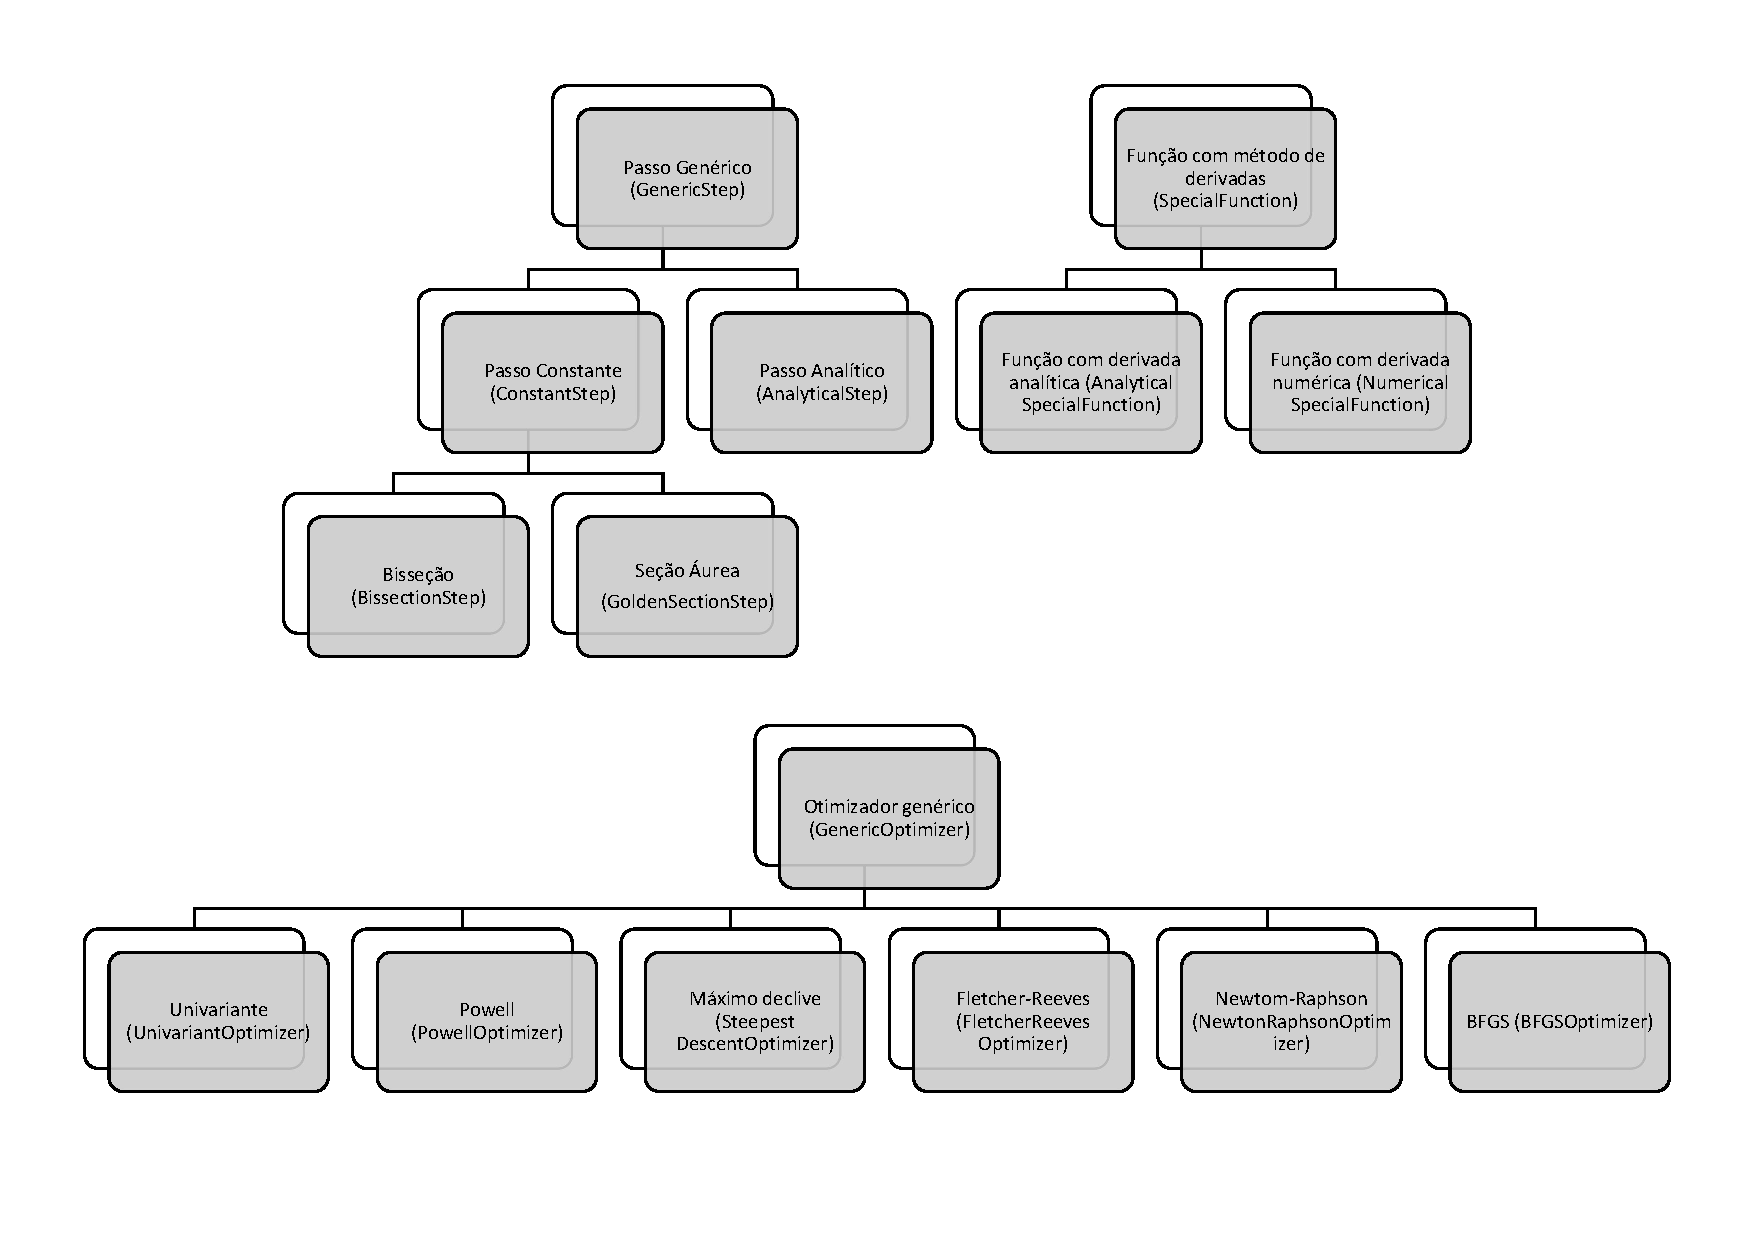
\includegraphics[width=0.8\textwidth]{../general/classes_full.pdf}
  \caption{Estrutura de classes implementada e heranças}
  \label{fig:q1_1}
\end{figure}

Como o principal objetivo do presente exercício é validar a implementação dos métodos de otimização e a função a ser estudada é sabidamente quadrática, dada uma direção de busca $\mathbf{d}_i$,
o valor do passo linear ideal $\alpha_i$ pode ser calculado com base no gradiente da função $\mathbf{\nabla}f$ e em sua Hessiana $\mathbf{H}(f)$ por meio da equação
\ref{eq:q1_1}.

\begin{equation}\label{eq:q1_1}
  \alpha_i = \frac{\mathbf{\nabla}f^T \mathbf{d}_i}{\mathbf{d}_i^T \mathbf{H}(f) \mathbf{d}_i}
\end{equation}

Para a função $f(x_1, x_2)$ descrita no enunciado, o gradiente e sua Hessiana são descritos nas equações \ref{eq:q1_2} e \ref{eq:q1_3}.

\begin{equation}\label{eq:q1_2}
  \mathbf{\nabla}f = \begin{bmatrix} 2x_1 - 3x_2 + 1\\-3x_1 + 8x_2 - 1 \end{bmatrix}
\end{equation}

\begin{equation}\label{eq:q1_3}
  \mathbf{H}(f) = \begin{bmatrix} 2 &-3 \\ -3 & 8 \end{bmatrix}
\end{equation}

Essa equação foi implementada como um objeto chamado {\tt AnalyticalStep} para ser passada aos métodos de otimização. O código desse objeto é mostrado abaixo:

\begin{python}
class AnalyticalStep(GenericStep):

  def __init__(self):

    super().__init__()

  def __call__(self, p_initial, direction, function):
    

    grad = function.grad(*p_initial).reshape(-1,1)
    direction = direction.reshape(-1,1)
    Q = function.Hessian(*p_initial)

    ak = - np.dot(grad.T, direction) / (direction.T @ Q @ direction)
    ak =  ak.reshape(-1)[0]

    pend = pend = p_initial + ak*direction.reshape(-1)

    return ak, pend
\end{python}

Ressalta-se que o critério de parada usado para os otimizadores foi o critério de parada aplicado para a otimização foi, no presente estudo, um limite de 3 iterações
e uma condção de chegada ao ponto crítico definida pela equação \ref{eq:q1_4}, com a tolerência $tol$ sendo igual a $10^{-5}$.

\begin{equation}\label{eq:q1_4}
  \left|\mathbf{\nabla}f\right| \leq tol
\end{equation}

Os resultados finais das 3 iterações executadas são resumidos na Tabela \ref{tab:results_summ}, com os resultados por passo em forma gráfica sendo mostrados na 
Figura \ref{fig:q1_2}. Nota-se a partir dos resultados que os valores finais obtidos foram coerentes com o previsto pela teoria, com os métodos Fletcher-Reeves,
Newton-Raphson e BFGS sendo os únicos a terem convergido no total de 3 passos ou menos, conforme esperado. Além disso, nota-se que o passo analítico para o método
de Newton-Raphson retornou também um valor de 1 na única iteração que este precisou, o que novamente está de acordo com o esperado pelo desenvolvimento teórico
do método. Também é interessante notar que os métodos de Powell e Univariante apresentaram passos iguais nas duas primeiras iterações, algo que novamente corrobora
com a boa implementação dos métodos dado que eles são idênticos nessas duas iterações.

\begin{table}[htpb]
  \centering
  \begin{tabular}{l|c|c|c|c|c|}
    Método             &	Ponto de mínimo	                     & Passos	 & $\alpha_1$   & $\alpha_2$	& $\alpha_3$ \\
    \hline
    Univariante        & $[ 1.093750,  1.062500,  2.256836]^T$ & 3       &  0.50000     & -0.93750    & -1.40625      \\
    Powell             & $[ 2.432024,  1.189955,  4.138784]^T$ & 3       &  0.50000     & -0.93750    & -0.13596      \\
    Steepest Descent   & $[ 0.484934,  0.320841,  0.344249]^T$ & 3       &  0.11647     &  0.70690    &  0.11648      \\
    Fletcher-Reeves    & $[-0.714286, -0.142857, -0.285714]^T$ & 2       &  0.11647     &  1.22648    &  --           \\
    Newton-Raphson     & $[-0.714286, -0.142857, -0.285714]^T$ & 1       &  1.00000     &  --         &  --           \\
    BFGS               & $[-0.714286, -0.142857, -0.285714]^T$ & 2       &  0.11647     &  1.22648    &  --           \\
    \hline
  \end{tabular}
  \caption{Resumo dos resultados obtidos}
  \label{tab:results_summ}
\end{table}


\begin{figure}[htpb]
  \centering
  \begin{subfigure}[b]{0.32\textwidth}
      \centering
      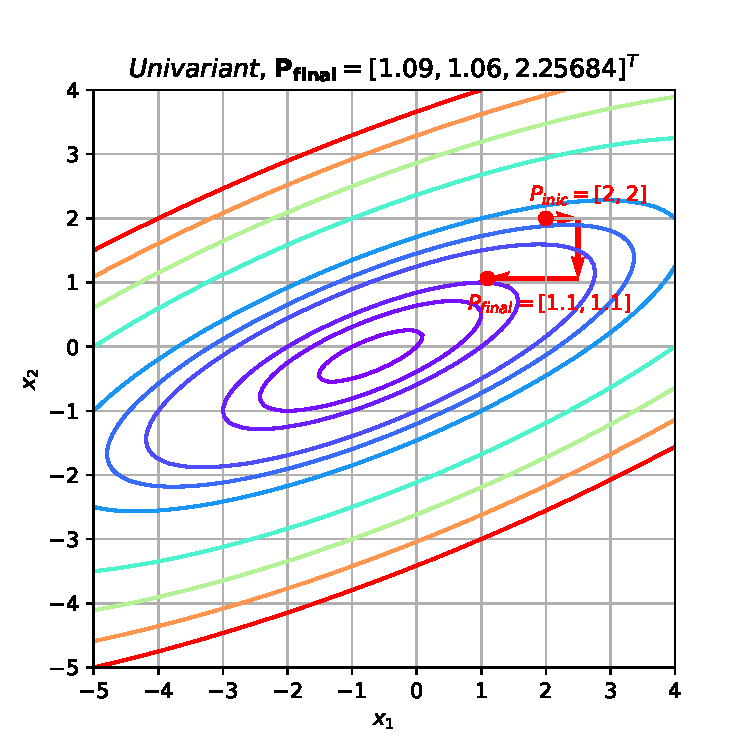
\includegraphics[width=\textwidth]{images/q1_Univariant.pdf}
      \caption{Univariante}
      \label{fig:q1_univariant}
  \end{subfigure}
  \hfill
  \begin{subfigure}[b]{0.32\textwidth}
    \centering
    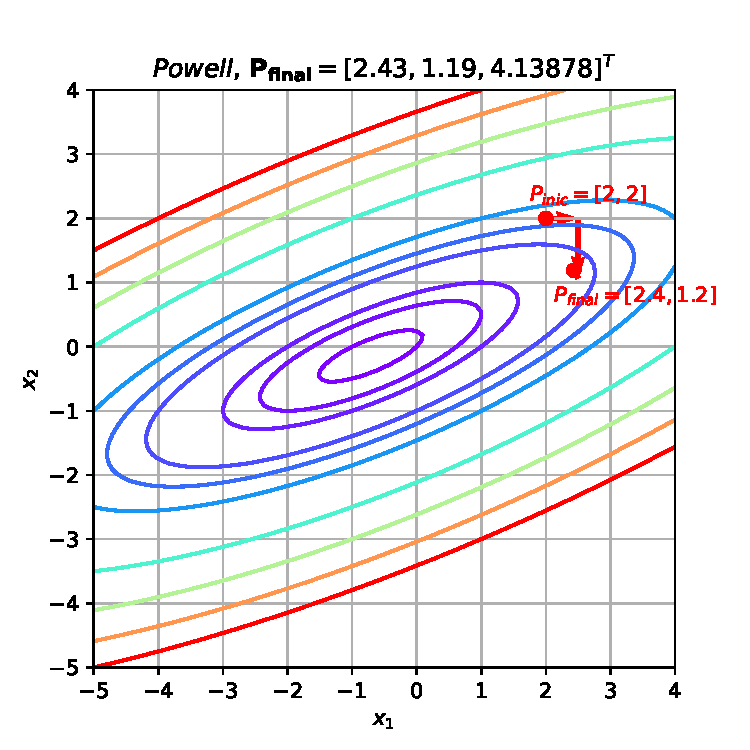
\includegraphics[width=\textwidth]{images/q1_Powell.pdf}
    \caption{Powell}
    \label{fig:q1_powell}
  \end{subfigure}
  \hfill
  \begin{subfigure}[b]{0.32\textwidth}
    \centering
    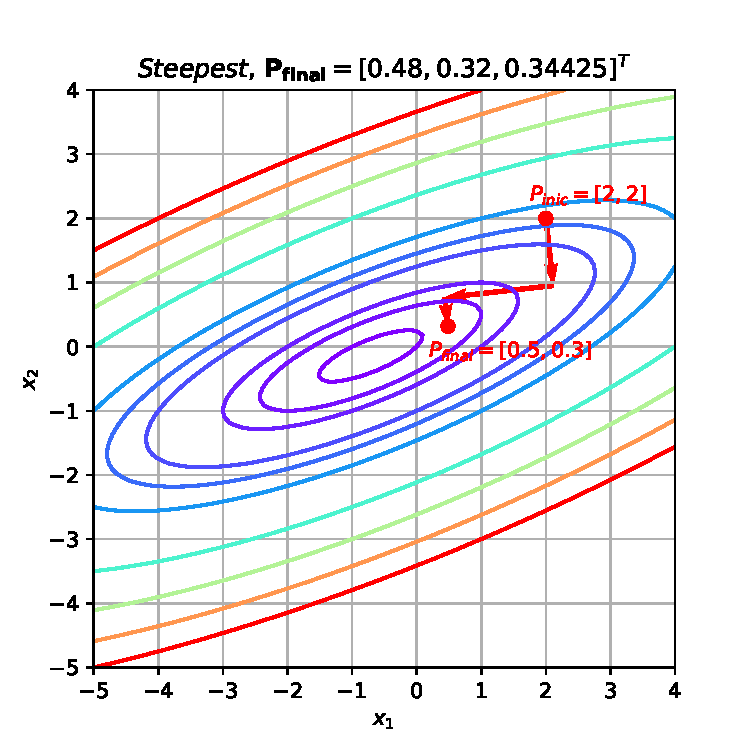
\includegraphics[width=\textwidth]{images/q1_Steepest.pdf}
    \caption{Steepest Descent}
    \label{fig:q1_steepest}
  \end{subfigure}
  \hfill
  \begin{subfigure}[b]{0.32\textwidth}
    \centering
    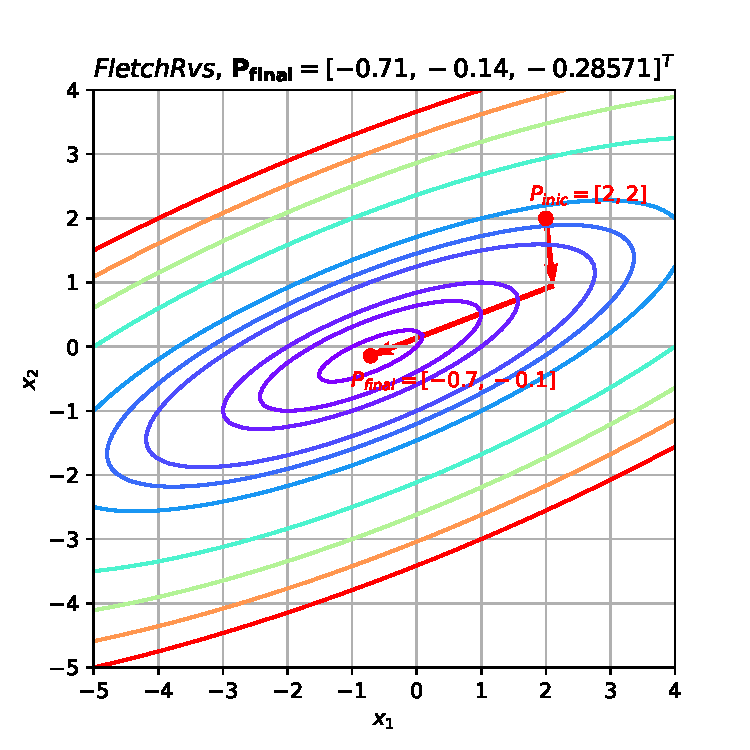
\includegraphics[width=\textwidth]{images/q1_FletchRvs.pdf}
    \caption{Fletcher-Reeves}
    \label{fig:q1_fletchrvs}
  \end{subfigure}
  \hfill
  \begin{subfigure}[b]{0.32\textwidth}
    \centering
    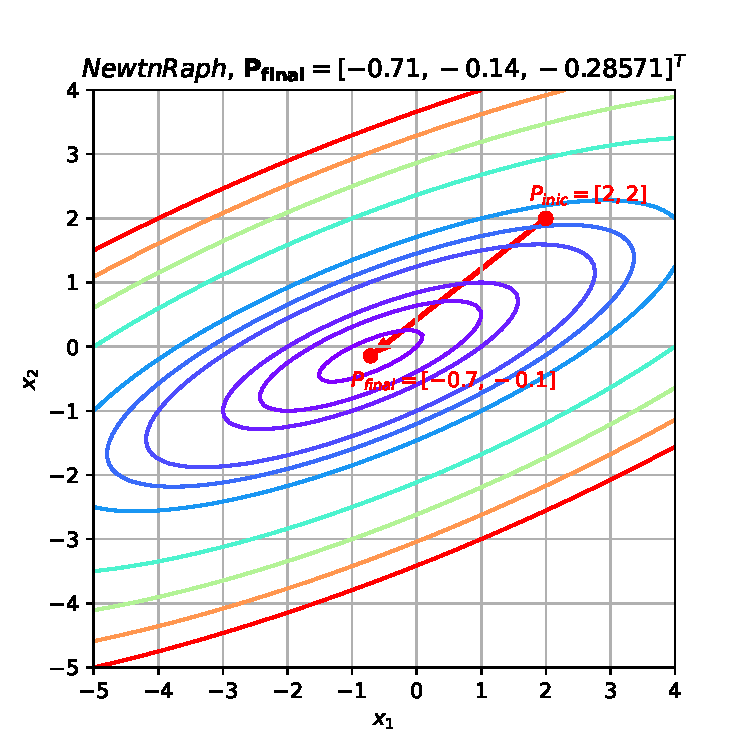
\includegraphics[width=\textwidth]{images/q1_NewtnRaph.pdf}
    \caption{Newton-Raphson}
    \label{fig:q1_newtnraph}
  \end{subfigure}
  \hfill
  \begin{subfigure}[b]{0.32\textwidth}
    \centering
    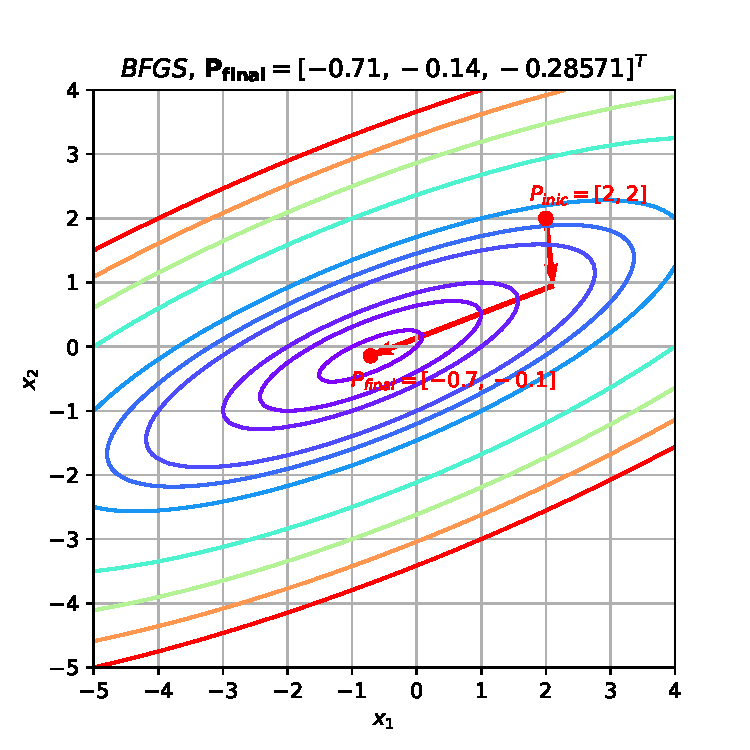
\includegraphics[width=\textwidth]{images/q1_BFGS.pdf}
    \caption{BFGS}
    \label{fig:q1_bfgs}
  \end{subfigure}
     \caption{Resumo gráfico dos passos dados em cada método}
     \label{fig:q1_2}
\end{figure}

%%%%%%%%%%%%%%%%%%%%%%%%%%%%%%%%%%%%%%%%%%%%%%%%%%%

\bibliographystyle{apalike}
\bibliography{export}

\end{document}